\section{mediamanagement Class Reference}
\label{classmediamanagement}\index{mediamanagement@{mediamanagement}}
{\tt \#include $<$mediamanagement.h$>$}

Inheritance diagram for mediamanagement:\begin{figure}[H]
\begin{center}
\leavevmode
\includegraphics[width=84pt]{classmediamanagement__inherit__graph}
\end{center}
\end{figure}
Collaboration diagram for mediamanagement:\begin{figure}[H]
\begin{center}
\leavevmode
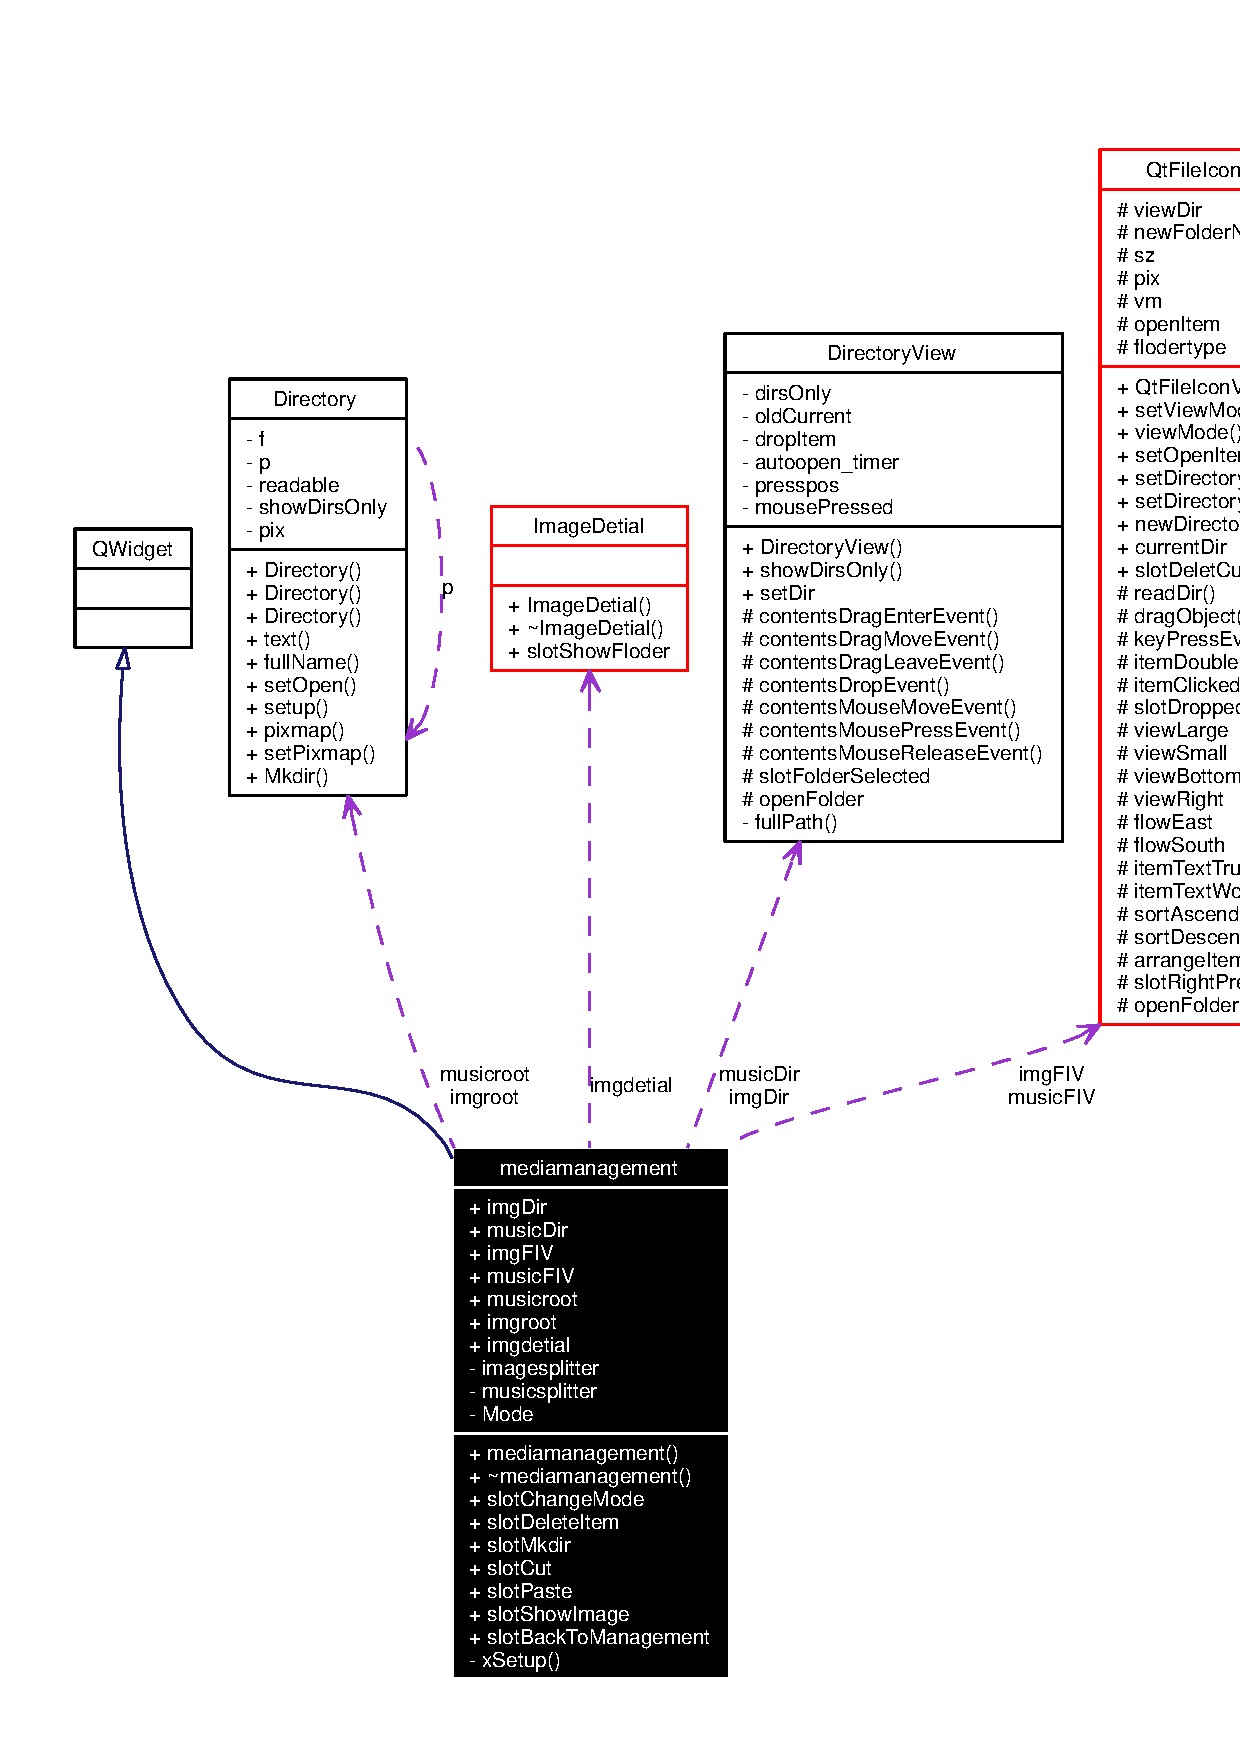
\includegraphics[width=320pt]{classmediamanagement__coll__graph}
\end{center}
\end{figure}


\subsection{Detailed Description}
\begin{Desc}
\item[Author:]root \end{Desc}




Definition at line 33 of file mediamanagement.h.\subsection*{Public Slots}
\begin{CompactItemize}
\item 
void {\bf slot\-Change\-Mode} (int)
\item 
void {\bf slot\-Delete\-Item} ()
\item 
void {\bf slot\-Mkdir} (QString dirname)
\item 
void {\bf slot\-Cut} ()
\item 
void {\bf slot\-Paste} ()
\item 
void {\bf slot\-Show\-Image} (KURL url)
\item 
void {\bf slot\-Back\-To\-Management} ()
\end{CompactItemize}
\subsection*{Signals}
\begin{CompactItemize}
\item 
void {\bf signal\-Image\-Detial} ()
\item 
void {\bf signal\-Show\-Keyboard} ()
\end{CompactItemize}
\subsection*{Public Member Functions}
\begin{CompactItemize}
\item 
{\bf mediamanagement} ({\bf QWidget} $\ast$parent=0, const char $\ast$name=0)
\item 
{\bf $\sim$mediamanagement} ()
\end{CompactItemize}
\subsection*{Public Attributes}
\begin{CompactItemize}
\item 
{\bf Directory\-View} $\ast$ {\bf img\-Dir}
\item 
{\bf Directory\-View} $\ast$ {\bf music\-Dir}
\item 
{\bf Qt\-File\-Icon\-View} $\ast$ {\bf img\-FIV}
\item 
{\bf Qt\-File\-Icon\-View} $\ast$ {\bf music\-FIV}
\item 
{\bf Directory} $\ast$ {\bf musicroot}
\item 
{\bf Directory} $\ast$ {\bf imgroot}
\item 
{\bf Image\-Detial} $\ast$ {\bf imgdetial}
\end{CompactItemize}
\subsection*{Private Member Functions}
\begin{CompactItemize}
\item 
void {\bf x\-Setup} ()
\end{CompactItemize}
\subsection*{Private Attributes}
\begin{CompactItemize}
\item 
QSplitter $\ast$ {\bf imagesplitter}
\item 
QSplitter $\ast$ {\bf musicsplitter}
\item 
int {\bf Mode}
\end{CompactItemize}


\subsection{Constructor \& Destructor Documentation}
\index{mediamanagement@{mediamanagement}!mediamanagement@{mediamanagement}}
\index{mediamanagement@{mediamanagement}!mediamanagement@{mediamanagement}}
\subsubsection{\setlength{\rightskip}{0pt plus 5cm}mediamanagement::mediamanagement ({\bf QWidget} $\ast$ {\em parent} = 0, const char $\ast$ {\em name} = 0)}\label{classmediamanagement_mediamanagementa0}




Definition at line 22 of file mediamanagement.cpp.

References x\-Setup().



\footnotesize\begin{verbatim}23  : QWidget(parent, name)
24 {
25     xSetup();
26 }
\end{verbatim}\normalsize 


Here is the call graph for this function:\begin{figure}[H]
\begin{center}
\leavevmode
\includegraphics[width=271pt]{classmediamanagement_mediamanagementa0_cgraph}
\end{center}
\end{figure}
\index{mediamanagement@{mediamanagement}!~mediamanagement@{$\sim$mediamanagement}}
\index{~mediamanagement@{$\sim$mediamanagement}!mediamanagement@{mediamanagement}}
\subsubsection{\setlength{\rightskip}{0pt plus 5cm}mediamanagement::$\sim${\bf mediamanagement} ()}\label{classmediamanagement_mediamanagementa1}




Definition at line 29 of file mediamanagement.cpp.



\footnotesize\begin{verbatim}30 {
31 }
\end{verbatim}\normalsize 


\subsection{Member Function Documentation}
\index{mediamanagement@{mediamanagement}!signalImageDetial@{signalImageDetial}}
\index{signalImageDetial@{signalImageDetial}!mediamanagement@{mediamanagement}}
\subsubsection{\setlength{\rightskip}{0pt plus 5cm}void mediamanagement::signal\-Image\-Detial ()\hspace{0.3cm}{\tt  [signal]}}\label{classmediamanagement_mediamanagementl0}




Definition at line 107 of file mediamanagement.moc.

Referenced by slot\-Show\-Image().



\footnotesize\begin{verbatim}108 {
109     activate_signal( staticMetaObject()->signalOffset() + 0 );
110 }
\end{verbatim}\normalsize 
\index{mediamanagement@{mediamanagement}!signalShowKeyboard@{signalShowKeyboard}}
\index{signalShowKeyboard@{signalShowKeyboard}!mediamanagement@{mediamanagement}}
\subsubsection{\setlength{\rightskip}{0pt plus 5cm}void mediamanagement::signal\-Show\-Keyboard ()\hspace{0.3cm}{\tt  [signal]}}\label{classmediamanagement_mediamanagementl1}




Definition at line 113 of file mediamanagement.moc.



\footnotesize\begin{verbatim}114 {
115     activate_signal( staticMetaObject()->signalOffset() + 1 );
116 }
\end{verbatim}\normalsize 
\index{mediamanagement@{mediamanagement}!slotBackToManagement@{slotBackToManagement}}
\index{slotBackToManagement@{slotBackToManagement}!mediamanagement@{mediamanagement}}
\subsubsection{\setlength{\rightskip}{0pt plus 5cm}void mediamanagement::slot\-Back\-To\-Management ()\hspace{0.3cm}{\tt  [slot]}}\label{classmediamanagement_mediamanagementi6}




Definition at line 248 of file mediamanagement.cpp.

References slot\-Change\-Mode().



\footnotesize\begin{verbatim}249 {
250         slotChangeMode(0);
251 }
\end{verbatim}\normalsize 
\index{mediamanagement@{mediamanagement}!slotChangeMode@{slotChangeMode}}
\index{slotChangeMode@{slotChangeMode}!mediamanagement@{mediamanagement}}
\subsubsection{\setlength{\rightskip}{0pt plus 5cm}void mediamanagement::slot\-Change\-Mode (int)\hspace{0.3cm}{\tt  [slot]}}\label{classmediamanagement_mediamanagementi0}




Definition at line 85 of file mediamanagement.cpp.

References imagesplitter, imgdetial, Mode, and musicsplitter.

Referenced by slot\-Back\-To\-Management(), and slot\-Show\-Image().



\footnotesize\begin{verbatim}86 {
87   //DAVID Set Mode
88   Mode=mode;
89   if (mode==0)//Image
90   {
91       imagesplitter->show();
92       musicsplitter->hide();
93       imgdetial->hide();
94   }
95   if(mode==1)
96   {
97       imagesplitter->hide();
98       musicsplitter->show();
99       imgdetial->hide();
100   }
101   if(mode==2)
102   {
103      imagesplitter->hide();
104      musicsplitter->hide();
105      imgdetial->show();
106   }
107 }
\end{verbatim}\normalsize 
\index{mediamanagement@{mediamanagement}!slotCut@{slotCut}}
\index{slotCut@{slotCut}!mediamanagement@{mediamanagement}}
\subsubsection{\setlength{\rightskip}{0pt plus 5cm}void mediamanagement::slot\-Cut ()\hspace{0.3cm}{\tt  [slot]}}\label{classmediamanagement_mediamanagementi3}




Definition at line 225 of file mediamanagement.cpp.

References Mode.



\footnotesize\begin{verbatim}226 {
227         if(Mode==0)//image
228         {
229                 qWarning("mediamanagement::slotCut()::image!!");
230         }
231         else if (Mode==1)//music
232         {
233                 qWarning("mediamanagement::slotCut()::music!!");
234         }
235 }
\end{verbatim}\normalsize 
\index{mediamanagement@{mediamanagement}!slotDeleteItem@{slotDeleteItem}}
\index{slotDeleteItem@{slotDeleteItem}!mediamanagement@{mediamanagement}}
\subsubsection{\setlength{\rightskip}{0pt plus 5cm}void mediamanagement::slot\-Delete\-Item ()\hspace{0.3cm}{\tt  [slot]}}\label{classmediamanagement_mediamanagementi1}




Definition at line 108 of file mediamanagement.cpp.

References Directory::full\-Name(), img\-Dir, img\-FIV, imgroot, Mode, music\-Dir, music\-FIV, musicroot, and Qt\-File\-Icon\-View::slot\-Delet\-Curr\-Item().



\footnotesize\begin{verbatim}109 {
110         //qWarning("MediaManagement::slotDeleteItem()");
111         //DAVID Check Mode
112         kdDebug()<<"Mode:"<<Mode;
113         if(Mode==0)//Image
114         {
115                  //check active area  musicDir or musicFIV
116                 //Delete Image Current QFileIconViewItem
117                 if(imgFIV->hasFocus())
118                 {
119                         qWarning("---------------1");
120                         imgFIV->slotDeletCurrItem();
121                         imgFIV->repaint();
122                 }
123                 else if(imgDir->hasFocus())
124                 {
125                         qWarning("----------------2");
126                         Directory *dir;
127                         for(dir=(Directory *)imgroot->firstChild();dir;dir=(Directory *)dir->nextSibling())
128                         {
129                           if(dir->isSelected())
130                           {
131                                 qWarning(dir->fullName());
132                                 QDir temp(dir->fullName());
133                                 const QFileInfoList* fileinfolist = temp.entryInfoList();
134                                 if(fileinfolist) 
135                                 {
136                                         QFileInfoListIterator it(*fileinfolist);
137                                         QFileInfo* fi;
138                                         while((fi = it.current()) != 0)
139                                         {
140                                                 if(fi->fileName() != "." && fi->fileName() != "..") 
141                                                 temp.remove(fi->absFilePath(),true);
142                                                 ++it;
143                                         }
144                                 }       
145                                 temp.cdUp();
146                                 temp.rmdir(dir->fullName());
147                                 //f.remove();
148                                 delete dir;
149                           }
150                         }
151                 }
152         }
153         else if(Mode==1)//music
154         {
155                 //Delete music Current QFileIconViewItem
156                 qWarning("Mode 1");
157                 if(musicFIV->hasFocus())
158                 {
159                         qWarning("----------------3");
160                         musicFIV->slotDeletCurrItem();
161                         musicFIV->repaint();
162                 }
163                 else if(musicDir->hasFocus())
164                 {
165                         qWarning("----------------4");
166                         Directory *dir;
167                         for(dir=(Directory *)musicroot->firstChild();dir;dir=(Directory *)dir->nextSibling())
168                         {
169                           if(dir->isSelected())
170                           {
171                                 qWarning(dir->fullName());
172                                 QDir temp(dir->fullName());
173                                 const QFileInfoList* fileinfolist = temp.entryInfoList();
174                                 if(fileinfolist) 
175                                 {
176                                         QFileInfoListIterator it(*fileinfolist);
177                                         QFileInfo* fi;
178                                         while((fi = it.current()) != 0)
179                                         {
180                                                 if(fi->fileName() != "." && fi->fileName() != "..") 
181                                                 temp.remove(fi->absFilePath(),true);
182                                                 ++it;
183                                         }
184                                 }       
185                                 temp.cdUp();
186                                 temp.rmdir(dir->fullName());
187                                 //f.remove();
188                                 delete dir;
189                           }
190                         }
191                         
192                 }
193         }
194 }
\end{verbatim}\normalsize 
\index{mediamanagement@{mediamanagement}!slotMkdir@{slotMkdir}}
\index{slotMkdir@{slotMkdir}!mediamanagement@{mediamanagement}}
\subsubsection{\setlength{\rightskip}{0pt plus 5cm}void mediamanagement::slot\-Mkdir (QString {\em dirname})\hspace{0.3cm}{\tt  [slot]}}\label{classmediamanagement_mediamanagementi2}




Definition at line 195 of file mediamanagement.cpp.

References img\-Dir, imgroot, Directory::Mkdir(), Mode, music\-Dir, and musicroot.



\footnotesize\begin{verbatim}196 {       
197         if(Mode==0)//Image
198         {
199                 //DAVID MKdir Current QFileIconViewItem
200                 qWarning("mediamanagement::slotMkdir()::Image!!!");
201                 imgroot->Mkdir(dirname);
202                 imgDir->repaint();
203                 
204         }
205         else if(Mode==1)//music
206         {
207                 //Delete music Current QFileIconViewItem
208                 qWarning("mediamanagement::slotMkdir()::music!!!");
209                 musicroot->Mkdir(dirname);
210                 musicDir->repaint();
211         }
212 }
\end{verbatim}\normalsize 
\index{mediamanagement@{mediamanagement}!slotPaste@{slotPaste}}
\index{slotPaste@{slotPaste}!mediamanagement@{mediamanagement}}
\subsubsection{\setlength{\rightskip}{0pt plus 5cm}void mediamanagement::slot\-Paste ()\hspace{0.3cm}{\tt  [slot]}}\label{classmediamanagement_mediamanagementi4}




Definition at line 214 of file mediamanagement.cpp.

References Mode.



\footnotesize\begin{verbatim}215 {
216         if(Mode==0)// image 
217         {
218                 qWarning("mediamanagement::slotPaste()::image");
219         }
220         else if(Mode==1)//music
221         {
222                 qWarning("mediamanagement::slotPaste()::music");
223         }
224 }
\end{verbatim}\normalsize 
\index{mediamanagement@{mediamanagement}!slotShowImage@{slotShowImage}}
\index{slotShowImage@{slotShowImage}!mediamanagement@{mediamanagement}}
\subsubsection{\setlength{\rightskip}{0pt plus 5cm}void mediamanagement::slot\-Show\-Image (KURL {\em url})\hspace{0.3cm}{\tt  [slot]}}\label{classmediamanagement_mediamanagementi5}




Definition at line 240 of file mediamanagement.cpp.

References signal\-Image\-Detial(), and slot\-Change\-Mode().

Referenced by x\-Setup().



\footnotesize\begin{verbatim}241 {
242         //Set Image
243         //DAVID change the mode to the image mode
244         slotChangeMode(2);
245         emit signalImageDetial();
246         
247 }
\end{verbatim}\normalsize 
\index{mediamanagement@{mediamanagement}!xSetup@{xSetup}}
\index{xSetup@{xSetup}!mediamanagement@{mediamanagement}}
\subsubsection{\setlength{\rightskip}{0pt plus 5cm}void mediamanagement::x\-Setup ()\hspace{0.3cm}{\tt  [private]}}\label{classmediamanagement_mediamanagementd0}




Definition at line 33 of file mediamanagement.cpp.

References imagesplitter, imgdetial, img\-Dir, img\-FIV, imgroot, Mode, music\-Dir, music\-FIV, musicroot, musicsplitter, Directory::set\-Open(), and slot\-Show\-Image().

Referenced by mediamanagement().



\footnotesize\begin{verbatim}34 {
35   //Initial here
36   //DAVID set backgorund color.
37   setPaletteBackgroundColor(QColor(0,0,0));
38   resize(750,500);
39   musicsplitter = new QSplitter( this );
40   
41   musicDir=new DirectoryView(musicsplitter,"MusicDir",true);
42   musicDir->addColumn( "Name" );
43   musicDir->setTreeStepSize( 40 );
44   musicroot = new Directory( musicDir, "/data/Media/MP3/" );
45   
46   musicroot->setOpen( TRUE );
47   musicsplitter->setResizeMode( musicDir, QSplitter::KeepSize );
48   musicFIV = new QtFileIconView( "/", musicsplitter );
49   musicFIV->setSelectionMode( QIconView::Extended );
50   musicsplitter->setGeometry(0,0,width(),height());
51   
52   
53    connect( musicDir, SIGNAL( folderSelected( const QString & ) ),
54              musicFIV, SLOT ( setDirectory( const QString & ) ) );
55 
57   imagesplitter = new QSplitter( this );
58   
59   imgDir=new DirectoryView(imagesplitter,"MusicDir",true);
60   imgDir->addColumn( "Name" );
61   imgDir->setTreeStepSize( 40 );
62   imgroot = new Directory( imgDir, "/data/Media/IMAGES/" );
63   
64   imgroot->setOpen( TRUE );
65   imagesplitter->setResizeMode( imgDir, QSplitter::KeepSize );
66   imgFIV = new QtFileIconView( "/", imagesplitter,"imgFIV",Image );
67   imgFIV->setSelectionMode( QIconView::Extended );
68   imagesplitter->setGeometry(0,0,width(),height());
69   imgdetial =new ImageDetial(this,"ImageDetail");
70   imgdetial->setGeometry(0,0,width(),height());
71   imgdetial->hide();
72   
73    connect( imgDir, SIGNAL( folderSelected( const QString & ) ),
74              imgFIV, SLOT ( setDirectory( const QString & ) ) );
75   
76   //DAVID Initial Album here    
77   //DAVID connect the show image singal to the ImageDetial
78   connect(imgFIV,SIGNAL(signalShowTheDetialofImage(KURL )),imgdetial,SLOT(slotShowFloder(KURL )));     
79   connect(imgFIV,SIGNAL(signalShowTheDetialofImage(KURL )),this,SLOT(slotShowImage(KURL )));
80   
81   imagesplitter->hide();
82 
83   Mode=1;            
84 }
\end{verbatim}\normalsize 


Here is the call graph for this function:\begin{figure}[H]
\begin{center}
\leavevmode
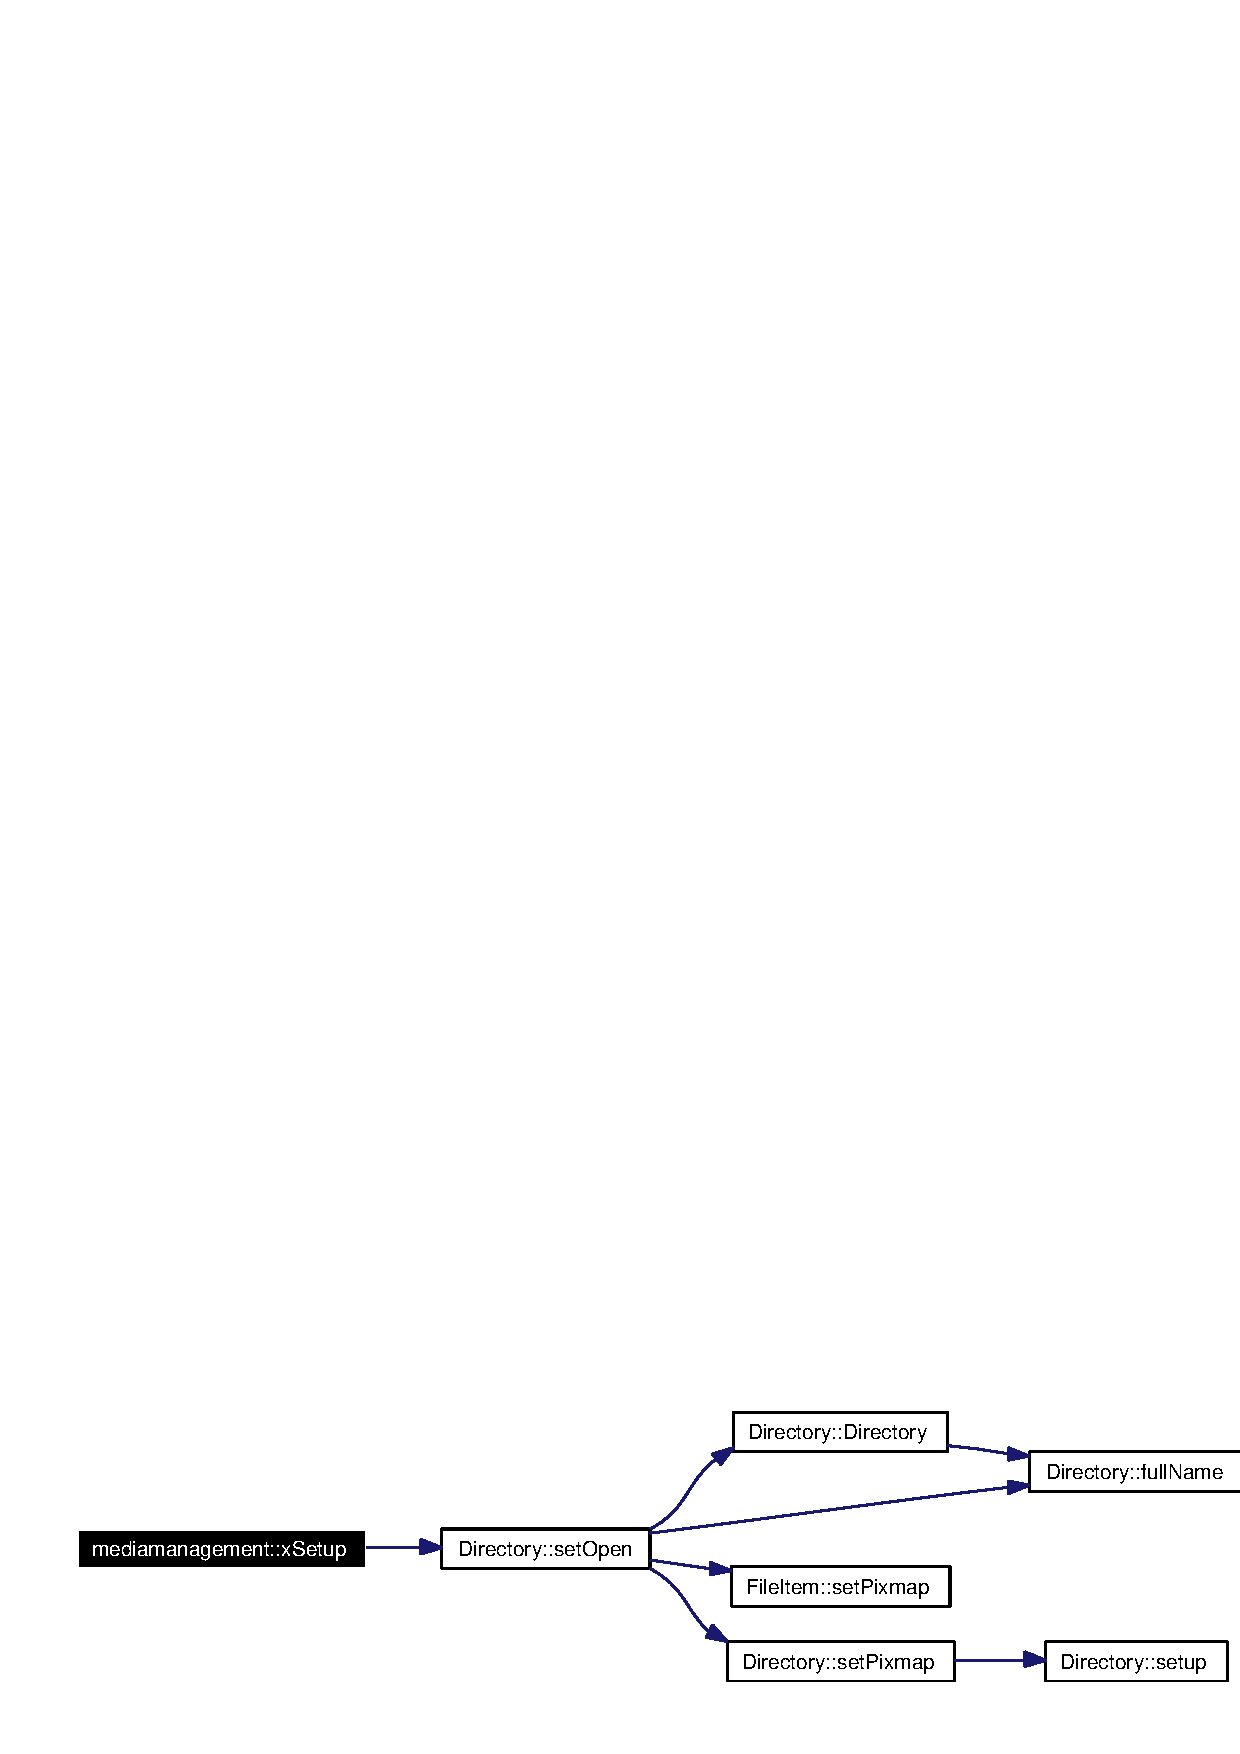
\includegraphics[width=298pt]{classmediamanagement_mediamanagementd0_cgraph}
\end{center}
\end{figure}


\subsection{Member Data Documentation}
\index{mediamanagement@{mediamanagement}!imagesplitter@{imagesplitter}}
\index{imagesplitter@{imagesplitter}!mediamanagement@{mediamanagement}}
\subsubsection{\setlength{\rightskip}{0pt plus 5cm}QSplitter$\ast$ {\bf mediamanagement::imagesplitter}\hspace{0.3cm}{\tt  [private]}}\label{classmediamanagement_mediamanagementr0}




Definition at line 58 of file mediamanagement.h.

Referenced by slot\-Change\-Mode(), and x\-Setup().\index{mediamanagement@{mediamanagement}!imgdetial@{imgdetial}}
\index{imgdetial@{imgdetial}!mediamanagement@{mediamanagement}}
\subsubsection{\setlength{\rightskip}{0pt plus 5cm}{\bf Image\-Detial}$\ast$ {\bf mediamanagement::imgdetial}}\label{classmediamanagement_mediamanagemento6}




Definition at line 44 of file mediamanagement.h.

Referenced by slot\-Change\-Mode(), x\-Setup(), and HDASS08::x\-Setup().\index{mediamanagement@{mediamanagement}!imgDir@{imgDir}}
\index{imgDir@{imgDir}!mediamanagement@{mediamanagement}}
\subsubsection{\setlength{\rightskip}{0pt plus 5cm}{\bf Directory\-View}$\ast$ {\bf mediamanagement::img\-Dir}}\label{classmediamanagement_mediamanagemento0}




Definition at line 39 of file mediamanagement.h.

Referenced by slot\-Delete\-Item(), slot\-Mkdir(), and x\-Setup().\index{mediamanagement@{mediamanagement}!imgFIV@{imgFIV}}
\index{imgFIV@{imgFIV}!mediamanagement@{mediamanagement}}
\subsubsection{\setlength{\rightskip}{0pt plus 5cm}{\bf Qt\-File\-Icon\-View}$\ast$ {\bf mediamanagement::img\-FIV}}\label{classmediamanagement_mediamanagemento2}




Definition at line 41 of file mediamanagement.h.

Referenced by slot\-Delete\-Item(), x\-Setup(), and HDASS08::x\-Setup().\index{mediamanagement@{mediamanagement}!imgroot@{imgroot}}
\index{imgroot@{imgroot}!mediamanagement@{mediamanagement}}
\subsubsection{\setlength{\rightskip}{0pt plus 5cm}{\bf Directory} $\ast$ {\bf mediamanagement::imgroot}}\label{classmediamanagement_mediamanagemento5}




Definition at line 43 of file mediamanagement.h.

Referenced by slot\-Delete\-Item(), slot\-Mkdir(), and x\-Setup().\index{mediamanagement@{mediamanagement}!Mode@{Mode}}
\index{Mode@{Mode}!mediamanagement@{mediamanagement}}
\subsubsection{\setlength{\rightskip}{0pt plus 5cm}int {\bf mediamanagement::Mode}\hspace{0.3cm}{\tt  [private]}}\label{classmediamanagement_mediamanagementr2}




Definition at line 59 of file mediamanagement.h.

Referenced by slot\-Change\-Mode(), slot\-Cut(), slot\-Delete\-Item(), slot\-Mkdir(), slot\-Paste(), and x\-Setup().\index{mediamanagement@{mediamanagement}!musicDir@{musicDir}}
\index{musicDir@{musicDir}!mediamanagement@{mediamanagement}}
\subsubsection{\setlength{\rightskip}{0pt plus 5cm}{\bf Directory\-View}$\ast$ {\bf mediamanagement::music\-Dir}}\label{classmediamanagement_mediamanagemento1}




Definition at line 40 of file mediamanagement.h.

Referenced by slot\-Delete\-Item(), slot\-Mkdir(), and x\-Setup().\index{mediamanagement@{mediamanagement}!musicFIV@{musicFIV}}
\index{musicFIV@{musicFIV}!mediamanagement@{mediamanagement}}
\subsubsection{\setlength{\rightskip}{0pt plus 5cm}{\bf Qt\-File\-Icon\-View}$\ast$ {\bf mediamanagement::music\-FIV}}\label{classmediamanagement_mediamanagemento3}




Definition at line 42 of file mediamanagement.h.

Referenced by slot\-Delete\-Item(), x\-Setup(), and HDASS08::x\-Setup().\index{mediamanagement@{mediamanagement}!musicroot@{musicroot}}
\index{musicroot@{musicroot}!mediamanagement@{mediamanagement}}
\subsubsection{\setlength{\rightskip}{0pt plus 5cm}{\bf Directory}$\ast$ {\bf mediamanagement::musicroot}}\label{classmediamanagement_mediamanagemento4}




Definition at line 43 of file mediamanagement.h.

Referenced by slot\-Delete\-Item(), slot\-Mkdir(), and x\-Setup().\index{mediamanagement@{mediamanagement}!musicsplitter@{musicsplitter}}
\index{musicsplitter@{musicsplitter}!mediamanagement@{mediamanagement}}
\subsubsection{\setlength{\rightskip}{0pt plus 5cm}QSplitter $\ast$ {\bf mediamanagement::musicsplitter}\hspace{0.3cm}{\tt  [private]}}\label{classmediamanagement_mediamanagementr1}




Definition at line 58 of file mediamanagement.h.

Referenced by slot\-Change\-Mode(), and x\-Setup().

The documentation for this class was generated from the following files:\begin{CompactItemize}
\item 
{\bf mediamanagement.h}\item 
{\bf mediamanagement.moc}\item 
{\bf mediamanagement.cpp}\end{CompactItemize}
